\documentclass[20pt,margin=1.5in,innermargin=-5.5in,blockverticalspace=-0.25in]{tikzposter}
\geometry{paperwidth=42in,paperheight=30in}
\usepackage[utf8]{inputenc}
\usepackage{amsmath}
\usepackage{amsfonts}
\usepackage{amsthm}
\usepackage{amssymb}
\usepackage{mathrsfs}
\usepackage{graphicx}
\usepackage{adjustbox}
\usepackage{enumitem}
\usepackage[backend=biber,style=numeric]{biblatex}
\usepackage{emory-theme}
\usepackage{hyperref}

\usepackage{mwe} % for placeholder images

\addbibresource{refs.bib}

% set theme parameters
\tikzposterlatexaffectionproofoff
\usetheme{EmoryTheme}
\usecolorstyle{EmoryStyle}

\title{Poster: Natural Logarithm of 2}
\author{Sarvesh Hiten Vora ID: 40081458}
\institute{Gina Cody School of Engineering and Computer Science, Concordia University\\}
\titlegraphic{
\includegraphics{CU_GCECS.jpeg}}

% begin document
\begin{document}
\maketitle
\centering
\begin{columns}
    \column{0.33}
    \block{Problem Statement:}{
         Let there be a calculator that computes the value of certain established irrational numbers. The purpose of the project is to carry out a number of activities, resulting in a set of interrelated artifacts for the problem domain of such a calculator.
         \\\textbf{ETERNITY:NUMBERS - Natural Logarithm of 2 $\ln(n)$.}
         \\\textbf{Knowledge State: } $\phi$
    }
    \block{Pre-Project Activity:}{
         \begin{enumerate}
             \item I have created a private GitHub repository called CalcUS.
             \item Added @mishanian Mishanian Ishanian as one of the Collaborators.
             \item Learnt basic Latex syntax to start with.
         \end{enumerate}
         \textbf{Knowledge State: } Knowledge State $\cup$ CalcUS $\cup$ Latex basic
         \\\textbf{Zeroth-order Ignorance - }Lack of Ignorance
    }
    \block{Problem 1 - Research \& Present Eternity:Number}{
       The irrational number Natural logarithm of 2 is very interesting number. Researching for it took really long time because the number is not well known.\\
       To understand the Eternity:Numbers, I had to go through various other aspect of mathematics for example understanding different kind of numbers and their properties, natural logarithm itself and Transcendental numbers. The whole understanding process was time consuming.\\
       Finding something unique about the given number was a big challenge. To achieve it I had to go through various resources and there was urge to get information from an experienced personnel.\\
       I have never worked with Latex before and It was a challenge to learn completely new language and implement it in short period of time.\\
       \textbf{Knowledge State: } Knowledge State $\cup$ Natural Log of 2 $\cup$ Latex first file
       \\\textbf{First-Order Ignorance - }Lack of Knowledge
    }
    \block{Problem 2 - Interview}{
        This problem consist of various tasks like generating interview questions, finding an interviewee, conducting an interview and finally concluding the interview.\\
        I was completely clueless at start but as I started thinking as a softwarement process it became clear.\\
        We first need some knowledge about the domain that we are going to work with. Hence, It was necessary to gather information.Generating questions for interview was easy since I was at first order of Ignorance level.
        \\Finding a proper interviewee was a bit of a concern because whenever I was approaching, due to the idea.
        But one of teaching faculties from my previous school accepted the proposal and I had conducted the interview. \\
        Still the information was not precise because there was a need for a domain expert. I was waiting for approval from Alexandros Mavrias, an investment analyst but the deadline approached \& I had to submit deliverable 1 without his interview. This was critical decision I made to submit the deliverable without his interview.
    }
    \column{0.34}
    \block{Problem 3 - Persona}{
        In this problem the challenge was to have same persona template across whole team. To overcome the challenge, we decided to have a brainstorming session where we can discuss and come up with various ideas to put into our persona template.\\
        The real issue arise when we come to know that the persona template we are trying to incorporate persona template file to out main .tex file because both had differnt Document Class and we can not have different document class in same .tex file. \\
        Solution, we decided to keep simple structure for persona rather than changing the whole document to make it look fancy.
    }
    
    \block{Problem 4 - Problem Domain Model}{
    The real challenge here was to identify and understand calculator domain.Hint, that has been given by professor in class to look into Wikipedia about it and search for the history helped allot.\\
    \vspace{1em}
        \begin{tikzfigure}[Natural Logarithm Of 2]
            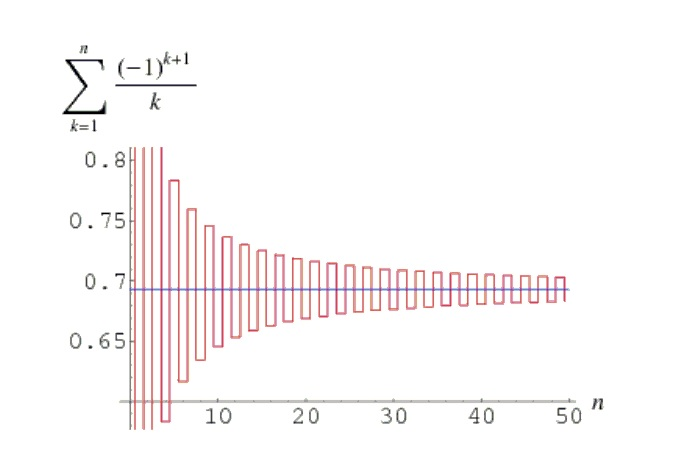
\includegraphics[width=0.9\linewidth]{Natural_log_2.jpeg}
        \end{tikzfigure}
    \vspace{1em}
    A calculator has various internal and external entities. Internal can be display and keyboard and external can be users or other advanced calculators that are used for a specific purpose.
    }
    \block{Problem 5 - Use case Model}{
    After identifying the problem domain, The next challenge was to construct various views of ETERNITY:NUMBERS using UML diagrams. Its really important to understand the question and work on it, that is where I made a mistake. It was important to put a normal scenario for each of the different views of system but I made a single normal scenario.\\
    I would have done it in much better way like understanding the question and coming up with various scenarios. Since my ETERNITY:NUMBERS was not having enough application to work with, I could not come up with different scenarios.
    
    }
    \column{0.33}
    \block{Problem 6 - User Story}{
        The challenge was to form an atomic user story that can be easily tested and implemented. To doing so, I required some more information. To gather those information I decided to take a survey of various kind of users of a calculator from different domain.\\
        I got an approval from Mr. Alexandros Mavrias, and I took his interview as well. The Challenge was where to put the survey and interview details to refer? I consult with TA and agreed upon putting those information in appendix and write a note about it. Fitting whole user story table on a single page was difficult, but then I decide to put only two column, one with identification number and another with all other details of a user story.\\
        \textbf{Knowledge State: } Knowledge State $\cup$ Application of Eternity:Numbers $\cup$ UML diagrams
    }
    \block{Problem 7 - Backward Traceability Matrix }{
    The actual challenge as mentioned in problem 6 was to fit the table on a single page, to achieve it I collapsed few columns into one as guided by TA.
    }
    \block{Problem 8 - Implementation in Java}{
    Since the user stories were quite atomic and straightforward, it was easy to implement them in Java.The important challenge was to decide whether to use Graphical UI or Text-based UI. It was a tough choice to make.\\
    As far as time was concerned, I preferred Text-based UI with plenty of instructions to operate calculator. This was a critical decision to make because in real world scenario we actually have tactical buttons to use.
    }
    
    \block{Conclusion}{
       If I analyse the \textbf{Knowledge State}, I can clearly see that the whole project was a good learning opportunity. At start the project was ambiguous but later on when pieces come together it became clear what to do and how to do it. Learning Latex and UML diagrams in detail was one of the positive outcome whereas managing time and resources was quite difficult. The importance of What approach over How approach is helpful. The project helped me to explore more about mathematics, moreover how to understand the domain and gather information to polish domain knowledge for specific application and correctly interpreting requirements of various stakeholders are fruitful gain from this project.
    }
    
    \block{References}{
        \vspace{-1em}
            Emory Theme for the tikzposter Author: Blair J. Rossetti\\
            Image taken from http://mathworld.wolfram.com/NaturalLogarithmof2.html
    }
\end{columns}
\end{document}